\documentclass[11pt,a4paper]{article}
\usepackage{stile}
\usepackage{graphicx}

\begin{document}
\documentotitolo{Manuale utente}{Alberi di regressione --- console e GUI}

Il manuale descrive l'avvio dei JAR da script su Windows e l'uso di console e GUI.
Per provare il training locale senza MySQL né server si può usare direttamente
la sezione \hyperref[sec:gui]{GUI}. La GUI richiede un ambiente desktop con Swing.

\section*{Prerequisiti}

Estrarre tutto il progetto in una cartella scrivibile, per esempio Documenti.
Non avviare i file dallo ZIP e mantenere la struttura di \texttt{distribution}.

\subsection*{Java su Windows}

Installare \textbf{Java 8 o successivo}, se non è già disponibile.
Gli script eseguono i JAR pronti: \textbf{non compilano il progetto e non
richiedono Eclipse o Maven}. Cercano Java prima in \texttt{JAVA\_HOME} e,
se questa variabile non è impostata, nel \texttt{PATH}.

Per configurare Java, cercare nel menu Start \textbf{Modifica le variabili di
ambiente per l'account}. Creare la variabile utente \texttt{JAVA\_HOME} con
il percorso della cartella del JDK, \textbf{senza virgolette e senza}
\texttt{\textbackslash bin}. Aprire un nuovo \textbf{Prompt dei comandi} e verificare:
\begin{lstlisting}
"%JAVA_HOME%\bin\java.exe" -version
\end{lstlisting}

In alternativa, senza \texttt{JAVA\_HOME}, deve funzionare \texttt{java -version}.
Se \texttt{JAVA\_HOME} è errata, correggerla oppure rimuoverla per usare il
\texttt{PATH}. Gli script non usano la configurazione Java di Eclipse.

\subsection*{MySQL: solo per l'apprendimento da database}

MySQL deve essere installato e in esecuzione sulla stessa macchina del server,
sulla porta \texttt{3306}. Prima del primo utilizzo, aprire in
\textbf{MySQL Workbench} una connessione locale con un account amministrativo;
con \textbf{File > Open SQL Script} aprire ed eseguire l'intero file:
\begin{lstlisting}
distribution/server/sql_file/map6_setup.sql
\end{lstlisting}

Il file crea \texttt{MapDB}, le tabelle \texttt{provaC} e \texttt{servo} e
l'utente \texttt{MapUser} con password \texttt{map}. Verificare che termini
senza errori. È per la \textbf{prima installazione}: non rieseguirlo su un
database già configurato senza controllarne il contenuto.
Gli script di avvio non installano né configurano MySQL.

\clearpage
\section*{Avvio su Windows}

Aprire la cartella \texttt{distribution} in Esplora file. Gli script sono:
\begin{itemize}
  \item \texttt{avvia-gui.bat}: esegue \texttt{gui/mapGUI.jar};
  \item \texttt{avvia-server.bat}: esegue \texttt{server/server.jar};
  \item \texttt{avvia-client.bat}: esegue \texttt{client/client\_base.jar};
  \item \texttt{avvia-locale.bat}: esegue \texttt{src/src.jar}, senza server.
\end{itemize}

\subsection*{Server}

Per apprendere da database, dopo aver preparato MySQL, fare doppio clic su
\texttt{avvia-server.bat}. Senza argomenti viene utilizzata la porta
\textbf{8080}. Lasciare aperta la finestra e avviare il client da console
oppure la GUI in modalità \textbf{Database}. Non fare doppio clic direttamente
sui JAR: gli script impostano la cartella di lavoro e lasciano visibili gli errori.

Lo script stampa un messaggio prima di eseguire Java; non è una verifica
che il servizio sia già pronto. Il server non stampa una conferma quando
inizia ad attendere connessioni: se il processo rimane attivo senza altri
messaggi, si può provare a collegare il client. Se invece compare un errore
o il messaggio \texttt{Esecuzione terminata}, il server non è in ascolto.

Gli alberi appresi vengono salvati in \texttt{distribution/server}, anche
se lo script è stato richiamato da un'altra cartella. Il driver
\path{mysql-connector-java-8.0.17.jar} deve rimanere accanto a \texttt{server.jar}.

\subsection*{Porta e indirizzo personalizzati}

Il doppio clic usa \texttt{localhost:8080}, adatto a server e client sullo
stesso computer. Per cambiare porta, aprire due Prompt dei comandi nella
cartella principale del progetto ed eseguire, prima nel primo e poi nel secondo:
\begin{lstlisting}
distribution\avvia-server.bat 9090
\end{lstlisting}
\begin{lstlisting}
distribution\avvia-client.bat localhost 9090
\end{lstlisting}

Se il server è su un altro computer, sostituire \texttt{localhost} con il suo
indirizzo IP e consentire la porta TCP nel firewall, sulla rete utilizzata.
Usare la stessa porta, fra \texttt{1} e \texttt{65535}, per server e client;
non confonderla con la \texttt{3306} di MySQL. \textbf{Nella GUI host e porta
si impostano nei campi della finestra}, non come argomenti di avvio.

In PowerShell usare il prefisso \texttt{.\textbackslash}, per esempio
\path{.\distribution\avvia-server.bat}.

\subsection*{Arresto}

Per arrestare il server premere \textbf{Ctrl+C} nella sua finestra e confermare
l'eventuale richiesta di terminare il processo batch. Gli script Windows
attendono la pressione di un tasto al termine dell'applicazione, anche in caso
di errore, per permettere di leggere i messaggi.

\clearpage
\section*{CLI}

La versione CLI utilizza il terminale per mostrare il menu, richiedere i dati e
visualizzare il risultato. Dopo ogni scelta digitata occorre premere Invio.
Negli esempi seguenti le righe in \textcolor{MAPinput}{blu} indicano l'input
dell'utente.

\subsection*{Client}

Con il server già avviato sulla porta 8080, fare doppio clic su
\path{distribution/avvia-client.bat}. Si apre una \textbf{seconda finestra},
collegata a \texttt{localhost:8080}. In alternativa, dal Prompt dei comandi
nella cartella principale del progetto:

\begin{lstlisting}
distribution\avvia-client.bat
\end{lstlisting}

Per un indirizzo o una porta diversi, passare gli argomenti allo script come
indicato nella sezione precedente. Il server va sempre avviato prima del client.

Una volta stabilita la connessione, il client presenta il menu:

\begin{lstlisting}
Learn Regression Tree from data [1]
Load Regression Tree from archive [2]
\end{lstlisting}
\didascalia{Menu principale del client da console.}

\begin{itemize}
  \item \textbf{1}: acquisisce gli esempi da una tabella del database e apprende
        un nuovo albero;
  \item \textbf{2}: carica dal disco del server un albero salvato in una
        precedente esecuzione.
\end{itemize}

\subsection*{Apprendimento da database}

Selezionare \textbf{1}. Alla richiesta \texttt{Table name:}, inserire il nome
della tabella da utilizzare, per esempio \texttt{provaC}.

\begin{lstlisting}
Learn Regression Tree from data [1]
Load Regression Tree from archive [2]
(*@\inpututente{1}@*)
Table name:
(*@\inpututente{provaC}@*)
Table found!
Starting data acquisition phase!
Starting learning phase!
\end{lstlisting}
\didascalia{Selezione della tabella e avvio dell'apprendimento.}

Dopo il caricamento dei dati, il server costruisce l'albero e lo salva nel file
\texttt{provaC.dmp}. Se l'operazione termina correttamente, il client passa
alla fase di predizione.

\clearpage
\subsection*{Predizione}

Durante questa fase il client mostra i rami disponibili nel nodo corrente.
Ogni riga contiene un indice e la condizione associata: per scegliere il ramo
occorre digitare il suo \textbf{indice numerico}, non il nome dell'attributo
o il valore da predire.

Nell'esempio con \texttt{provaC}, il primo nodo distingue i valori
\texttt{A} e \texttt{B} dell'attributo \texttt{X}:

\begin{lstlisting}
Starting prediction phase!
0:X=A
1:X=B
(*@\inpututente{0}@*)
\end{lstlisting}
\didascalia{Scelta del ramo corrispondente a X=A.}

Se il ramo selezionato conduce a un altro nodo interno, viene presentata una
nuova domanda. Il numero di scelte dipende dal percorso seguito nell'albero.
Proseguendo nell'esempio:

\begin{lstlisting}
0:Y<=2.0
1:Y>2.0
(*@\inpututente{0}@*)
\end{lstlisting}
\didascalia{Seconda scelta: il ramo in cui Y è minore o uguale a 2.0.}

Raggiunta una foglia, il client mostra il valore predetto, preceduto dal
messaggio \texttt{Predicted class:}. Per le scelte indicate il risultato è
\texttt{1.0}.

\begin{lstlisting}
Predicted class:1.0
Would you repeat ? (y/n)
\end{lstlisting}
\didascalia{Risultato della predizione e richiesta di ripetizione.}

Alla domanda finale:
\begin{itemize}
  \item digitare \textbf{y} per iniziare una nuova predizione sullo stesso
        albero, ripartendo dalla radice;
  \item digitare \textbf{n} per terminare il client.
\end{itemize}

La chiusura del client non arresta il server, che resta disponibile per altre
connessioni.

\clearpage
\subsection*{Caricamento da archivio}

L'opzione \textbf{2} del menu iniziale permette di riutilizzare un albero già
salvato. Prima di selezionarla deve quindi essere disponibile un archivio
prodotto dal server, per esempio \texttt{provaC.dmp} dopo l'apprendimento
descritto nelle pagine precedenti.

Il file deve trovarsi nella directory di lavoro del server. Se il servizio è
stato avviato con gli script di questo manuale, tale directory è
\texttt{distribution/server}. L'archivio non va cercato nella cartella del
client.

Avviare nuovamente il client, selezionare \textbf{2} e rispondere alla richiesta
\texttt{File name:} inserendo il nome \textbf{senza l'estensione}
\texttt{.dmp}:

\begin{lstlisting}
Learn Regression Tree from data [1]
Load Regression Tree from archive [2]
(*@\inpututente{2}@*)
File name:
(*@\inpututente{provaC}@*)
Table found!
Starting prediction phase!
\end{lstlisting}
\didascalia{Caricamento dell'albero conservato in provaC.dmp.}

Il messaggio \texttt{Table found!} viene utilizzato dal programma anche per
confermare il caricamento di un archivio. Non viene eseguito un nuovo
apprendimento: la predizione utilizza l'albero letto dal file.

Le scelte si effettuano con la stessa procedura già descritta. Nell'esempio,
selezionando il ramo \texttt{1}, corrispondente a \texttt{X=B}, si raggiunge
una foglia con valore \texttt{10.0}:

\begin{lstlisting}
0:X=A
1:X=B
(*@\inpututente{1}@*)
Predicted class:10.0
Would you repeat ? (y/n)
(*@\inpututente{n}@*)
\end{lstlisting}
\didascalia{Predizione sull'albero caricato e chiusura del client.}

Anche dopo il caricamento è possibile rispondere \textbf{y} per ripetere la
predizione oppure \textbf{n} per terminare.

\clearpage
\section*{GUI}
\phantomsection\label{sec:gui}

L'interfaccia grafica permette di apprendere e visualizzare l'intero albero.
Non occorre rispondere alle domande della console: le condizioni e i valori
predetti sono mostrati direttamente nel grafico.

\subsection*{Avvio e primo training locale}

Aprire un terminale nella \textbf{cartella principale del progetto} ed eseguire:

\begin{lstlisting}
java -jar distribution/gui/mapGUI.jar
\end{lstlisting}

Si apre la finestra \textbf{Progetto Map 2026}. All'inizio è selezionata
l'origine \textbf{File locale}, la barra di stato indica \textbf{Pronto} e
l'area centrale mostra \textbf{In attesa del training}.

\begin{enumerate}
  \item Lasciare selezionato \textbf{File locale}.
  \item Nel campo \textbf{Training set} mantenere il percorso predefinito
        \path{distribution/src/prova.dat}. In alternativa premere
        \textbf{Scegli file} e selezionare un training set \texttt{.dat}.
  \item Premere \textbf{Avvia training} e attendere il risultato. Non è
        necessario avviare il server o installare MySQL per questa modalità.
\end{enumerate}

\begin{center}
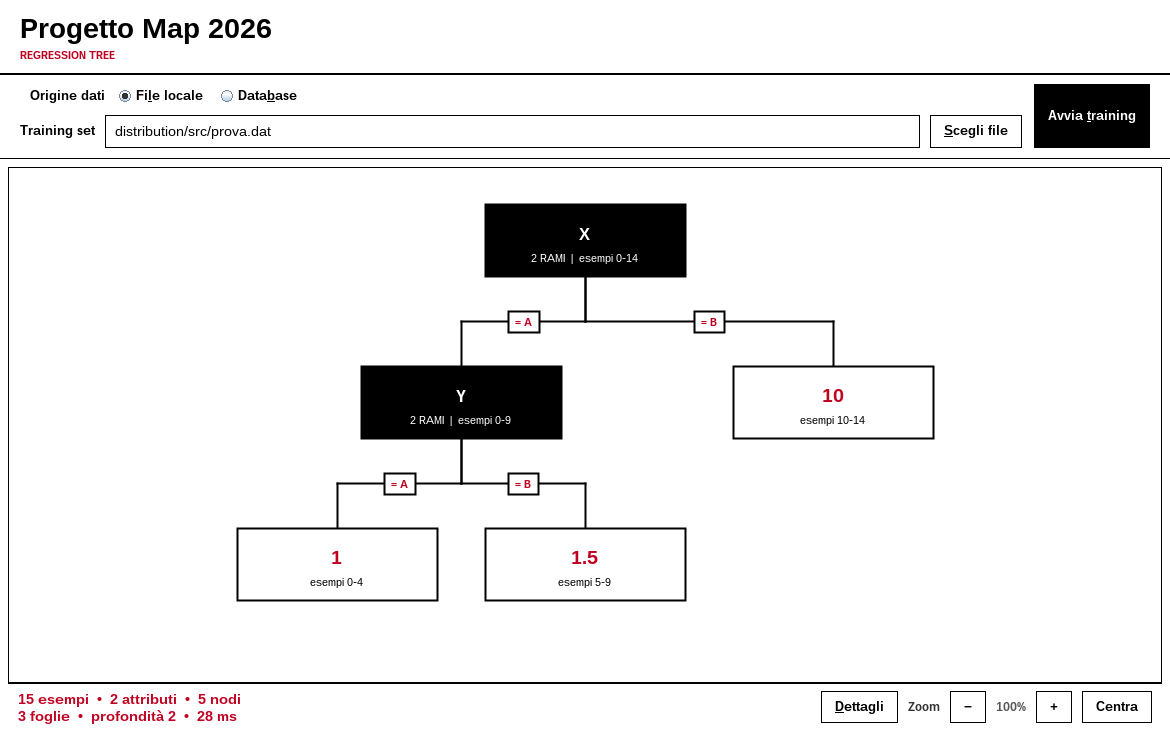
\includegraphics[width=\textwidth]{immagini/gui-locale.png}
\end{center}
\didascalia{GUI dopo il training locale su prova.dat. L'aspetto dei controlli
può variare con il sistema operativo; il tempo visualizzato dipende dalla macchina.}

Per questo file il risultato comprende \textbf{15 esempi}, \textbf{2 attributi},
\textbf{5 nodi}, \textbf{3 foglie} e \textbf{profondità 2}. Il pulsante
\textbf{Dettagli} diventa disponibile. Se il percorso predefinito non viene
trovato, avviare il programma dalla cartella principale oppure scegliere il
file tramite il selettore, che inserisce il percorso assoluto.

\clearpage
\subsection*{Lettura dell'albero e dei risultati}

L'albero si legge dall'alto verso il basso. I rettangoli \textbf{neri}
rappresentano gli attributi su cui si effettuano le scelte. I rettangoli
\textbf{bianchi}, con il valore numerico in rosso, sono le foglie e contengono
la predizione. Le etichette sui collegamenti indicano la condizione da seguire.

Per il file locale \texttt{prova.dat}, gli attributi \texttt{X} e \texttt{Y}
sono discreti. Le predizioni si leggono così:

\begin{center}
\begin{tabularx}{\textwidth}{@{}Xr@{}}
\toprule
\textbf{Percorso} & \textbf{Valore predetto} \\
\midrule
\texttt{X=A}, poi \texttt{Y=A} & 1 \\
\texttt{X=A}, poi \texttt{Y=B} & 1.5 \\
\texttt{X=B} & 10 \\
\bottomrule
\end{tabularx}
\end{center}

Il grafico è una \textbf{visualizzazione}, non un modulo di inserimento per
nuovi esempi: i nodi non sono pulsanti e non si selezionano con un clic.
Per una predizione guidata tramite domande usare il client da console.
I valori delle foglie sono mostrati con al massimo quattro cifre decimali.

\subsection*{Comandi di consultazione}

\begin{center}
\begin{tabularx}{\textwidth}{@{}lX@{}}
\toprule
\textbf{Comando} & \textbf{Effetto} \\
\midrule
\textbf{Dettagli} & Apre la finestra \textbf{Dettagli albero} con la
rappresentazione testuale del risultato. È disponibile dopo un training riuscito. \\
\textbf{Zoom -- / +} & Riduce o aumenta lo zoom di 10 punti percentuali,
fra 50\% e 150\%. La percentuale corrente è indicata accanto ai pulsanti. \\
\textbf{Centra} & Riporta la vista verso la radice, in alto. Non adatta
l'intero albero alla finestra e non reimposta lo zoom. \\
\textbf{Barre di scorrimento} & Permettono di esplorare gli alberi che
superano l'area visibile. Compaiono quando necessarie. \\
\bottomrule
\end{tabularx}
\end{center}

La barra inferiore riporta nodi, foglie, profondità e tempo impiegato.
La profondità è il numero massimo di collegamenti dalla radice a una foglia:
un albero formato da una sola foglia ha profondità zero. Il tempo indicato
non è una stima del tempo restante.

In modalità locale sono mostrati anche numero di esempi e attributi. La
scritta \texttt{esempi 0-14}, per esempio, indica un intervallo di indici nei
dati elaborati: durante il training gli esempi vengono riordinati, quindi non
si tratta dei numeri di riga originali del file.

Per apprendere un altro albero, cambiare file oppure origine e premere
nuovamente \textbf{Avvia training}. Il nuovo risultato sostituisce quello
precedente; il semplice cambio dell'origine non avvia alcuna elaborazione.

\clearpage
\subsection*{Training da database}

Questa modalità richiede MySQL configurato e il \textbf{server MAP già
avviato}, come descritto all'inizio del manuale. La GUI comunica con il server
MAP: non si collega direttamente alla porta MySQL e non richiede credenziali
del database nella finestra.

\begin{enumerate}
  \item Selezionare \textbf{Database} in \textbf{Origine dati}.
  \item Nel campo \textbf{Tabella} inserire \texttt{provaC}, oppure il nome
        di un'altra tabella compatibile già presente in \texttt{MapDB}.
        Non inserire un percorso, un comando SQL o il suffisso \texttt{.dat}.
  \item Nel campo \textbf{Server MAP} inserire \texttt{localhost} se il
        server è sullo stesso computer; altrimenti usare il suo indirizzo.
  \item Nel campo accanto ai due punti inserire la porta del server MAP,
        normalmente \texttt{8080}, \textbf{non 3306}, che è la porta MySQL.
  \item Premere \textbf{Avvia training} e attendere la comparsa dell'albero.
\end{enumerate}

\begin{center}
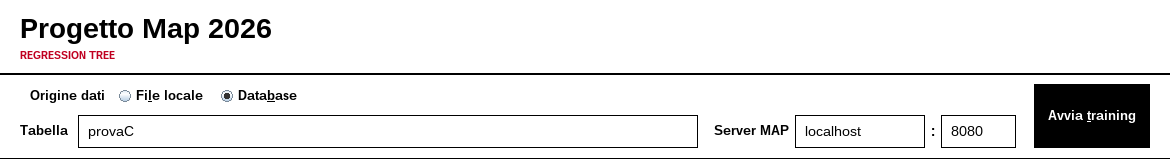
\includegraphics[width=\textwidth]{immagini/gui-database.png}
\end{center}
\didascalia{Pannello di configurazione dell'origine Database con i valori predefiniti.}

La tabella deve avere un nome che inizia con una lettera; i caratteri
successivi possono essere lettere, cifre, underscore o dollaro. La porta deve
essere un intero fra 1 e 65535. La configurazione JDBC del server usa
\texttt{localhost:3306/MapDB}, utente \texttt{MapUser} e password \texttt{map},
coerentemente con lo script di prima installazione fornito.

Al termine, la barra riporta tabella, server, numero di nodi e foglie,
profondità e tempo. Non mostra il numero degli esempi e degli attributi,
perché queste informazioni non vengono trasferite dal protocollo remoto.
\textbf{Dettagli} visualizza il nome della tabella e la struttura ricostruita.

\subsection*{Esempio con la tabella provaC}

Nella tabella \texttt{provaC} fornita dallo script, \texttt{X} è discreto e
\texttt{Y} è numerico. Diversamente da \texttt{prova.dat}, il secondo split
utilizza una soglia:

\begin{center}
\begin{tabularx}{\textwidth}{@{}Xr@{}}
\toprule
\textbf{Percorso} & \textbf{Valore predetto} \\
\midrule
\texttt{X=A}, poi \texttt{Y<=2.0} & 1 \\
\texttt{X=A}, poi \texttt{Y>2.0} & 1.5 \\
\texttt{X=B} & 10 \\
\bottomrule
\end{tabularx}
\end{center}

Il server salva automaticamente \texttt{provaC.dmp} nella propria directory
di lavoro, sovrascrivendo l'eventuale archivio omonimo. La GUI non salva una
copia sul computer del client e non permette di aprire direttamente gli
archivi: per riutilizzarli senza apprendere di nuovo, usare l'opzione
\textbf{2} della CLI.

\clearpage
\subsection*{Formato dei training set locali}

\textbf{Scegli file} seleziona un dataset di testo \texttt{.dat}, non un albero
serializzato \texttt{.dmp} e non un file CSV generico privo di schema.
Il seguente esempio riproduce il contenuto di \texttt{prova.dat} distribuito:

\begin{lstlisting}
@schema 2
@desc X A,B,C,D,E
@desc Y A,B,C,D,E
@target class
@data 15
A,A,1
A,A,1
A,A,1
A,A,1
A,B,1.5
A,B,1.5
A,B,1.5
B,B,10
A,B,1.5
A,B,1.5
B,C,10
B,B,10
B,C,10
B,C,10
A,A,1
\end{lstlisting}

\begin{itemize}
  \item \texttt{@schema 2} indica due attributi descrittivi, escluso il target.
  \item Ogni \texttt{@desc} dichiara un attributo. L'elenco separato da
        virgole specifica il dominio discreto; senza elenco l'attributo è
        continuo. Per esempio, \texttt{@desc Y} dichiara \texttt{Y} numerico.
  \item \texttt{@target class} dichiara il nome del target numerico,
        collocato nell'ultima colonna di ogni riga.
  \item \texttt{@data 15} dichiara esattamente quindici esempi. Ogni riga
        contiene i valori degli attributi nell'ordine dello schema, poi
        il target; i campi sono separati da virgole.
\end{itemize}

Usare il \textbf{punto} come separatore decimale, rispettare maiuscole e
minuscole dei valori discreti e non aggiungere righe vuote o commenti.
Nelle dichiarazioni usare un singolo spazio fra i campi, come nell'esempio.
Il numero di righe e quello delle colonne devono coincidere con lo schema.

Sono disponibili anche \path{distribution/src/provaC.dat}, con un
attributo continuo, e \path{distribution/src/servo.dat}, più ampio.
I file non vengono modificati dal training. La modalità locale conserva il
risultato soltanto in memoria e non crea un archivio \texttt{.dmp}.

\subsection*{Chiusura}

Chiudere la finestra per terminare la GUI. Il risultato locale non viene
salvato automaticamente; se serve nuovamente, ripetere il training sul file.
Il server MAP resta attivo anche dopo la chiusura della GUI o della CLI:
per arrestarlo, premere \textbf{Ctrl+C} nel suo terminale.


\clearpage
\section*{Applicazione locale da console: senza MySQL}

Per usare i dataset su file, senza server né GUI, aprire la cartella
\texttt{distribution} e fare doppio clic su \texttt{avvia-locale.bat}.
Dal Prompt dei comandi nella cartella principale del progetto:
\begin{lstlisting}
distribution\avvia-locale.bat
\end{lstlisting}

Lo script esegue \texttt{src/src.jar} con directory di lavoro
\texttt{distribution/src}, dove sono già presenti \texttt{prova.dat},
\texttt{provaC.dat} e \texttt{servo.dat}.

\begin{enumerate}
  \item Scegliere \textbf{1} per apprendere un albero e, alla richiesta
        \texttt{File name:}, digitare per esempio \texttt{provaC},
        \textbf{senza} \texttt{.dat}.
  \item Il programma legge il dataset, salva \texttt{provaC.dmp} nella stessa
        cartella e stampa le regole dell'albero.
  \item Per la predizione scegliere gli indici numerici dei rami proposti.
        Il valore predetto viene stampato a video; rispondere \textbf{y} per
        ripetere oppure \textbf{n} per terminare.
  \item A un avvio successivo, scegliere \textbf{2} e digitare
        \texttt{provaC}, senza \texttt{.dmp}, per caricare l'albero salvato.
\end{enumerate}

Gli archivi del server e della console locale \textbf{non sono intercambiabili}:
mantenerli nelle rispettive cartelle. Diversamente da questa console, la GUI
locale richiede il percorso completo di estensione \texttt{.dat} e non salva
archivi \texttt{.dmp}.

\section*{Eclipse e JAR distribuiti}

Per provare i JAR usare gli script da Esplora file o dal terminale, anche quando
Eclipse è installato. Non occorre importare i progetti.

Solo per consultare o modificare i sorgenti della base, in Eclipse scegliere
\textbf{File > Import > General > Existing Projects into Workspace}, selezionare
\texttt{project} e abilitare \textbf{Search for nested projects}. Importare
\texttt{mapClient}, \texttt{mapServer} e \texttt{src} senza selezionare
\textbf{Copy projects into workspace}, così da mantenere il collegamento al
driver JDBC in \texttt{distribution/server}.

Per compilare serve un JDK compatibile con la versione dell'IDE.
In \textbf{Window > Preferences > Java > Installed JREs} aggiungere il JDK;
in \textbf{Java > Installed JREs > Execution Environments} associarlo a
\texttt{JavaSE-1.8}. Questa impostazione non modifica \texttt{JAVA\_HOME}
o il \texttt{PATH} usati dagli script.

La cartella \texttt{estensioni/gui} contiene i sorgenti Swing, ma non è un
progetto Eclipse già configurato. La GUI usa la base locale
\texttt{project/src/src}, non le classi omonime del server;
\texttt{mapGUI.jar} contiene già quanto serve alla sua esecuzione.

\textbf{Run As > Java Application} esegue le classi compilate da Eclipse,
non i JAR. Dopo una modifica ai sorgenti, gli script continuano a eseguire i
vecchi JAR finché questi non vengono esportati nuovamente.

\clearpage
\section*{Linux e macOS}

Gli equivalenti \texttt{.sh} hanno gli stessi valori predefiniti, argomenti e
directory di lavoro dei \texttt{.bat}. Serve Java 8 o successivo tramite
\texttt{JAVA\_HOME} oppure \texttt{PATH}; la GUI richiede un ambiente desktop.

Dalla cartella principale del progetto, per la GUI locale:
\begin{lstlisting}
sh distribution/avvia-gui.sh
\end{lstlisting}
Per apprendere da database, preparare MySQL e avviare prima il server:
\begin{lstlisting}
sh distribution/avvia-server.sh
\end{lstlisting}
Poi, in un secondo terminale, avviare la GUI e scegliere \textbf{Database},
oppure usare il client da console:
\begin{lstlisting}
sh distribution/avvia-client.sh
\end{lstlisting}
Per una porta diversa o un altro indirizzo, in terminali separati:
\begin{lstlisting}
sh distribution/avvia-server.sh 9090
sh distribution/avvia-client.sh localhost 9090
\end{lstlisting}
Nella GUI impostare gli stessi host e porta nei campi della finestra.
Per la sola applicazione locale da console:
\begin{lstlisting}
sh distribution/avvia-locale.sh
\end{lstlisting}
Gli script \texttt{.sh} non attendono un tasto al termine. Per interrompere
il server utilizzare \textbf{Ctrl+C}; per la GUI chiudere la finestra grafica.

\section*{Problemi comuni}

\begin{description}[style=nextline,leftmargin=0pt]
  \item[Java non trovato o JAVA\_HOME non valida.]
    Controllare \texttt{JAVA\_HOME} e \texttt{PATH} e riaprire il terminale.
    L'errore \texttt{UnsupportedClassVersionError} indica Java troppo vecchio:
    usare almeno Java 8 per i JAR forniti.
  \item[JAR mancante, GUI non visibile o dataset non trovato.]
    Mantenere la struttura della distribuzione. La GUI richiede un desktop
    con supporto Swing; controllare gli errori nella console. Usare
    \textbf{Scegli file} per selezionare un dataset completo di \texttt{.dat}.
  \item[Errore di connessione, porta occupata o tabella non trovata.]
    Avviare prima il server e verificare host, porta e firewall.
    \texttt{Address already in use} indica una porta occupata: chiudere l'altra
    istanza o cambiare porta anche nel client o nella GUI.
    Per il training da database controllare MySQL su \texttt{localhost:3306},
    \texttt{MapDB}, l'utente \texttt{MapUser} e l'esito dello script SQL.
  \item[Archivio non trovato o salvataggio non riuscito.]
    Il server salva in \texttt{distribution/server}; la console locale in
    \texttt{distribution/src}. Inserire i nomi senza \texttt{.dmp} e verificare
    che l'archivio sia già stato generato e la cartella sia scrivibile.
    La GUI locale non salva né apre archivi.
\end{description}

\end{document}
